%% ============================================================
%%  SECTION 5 — KỊCH BẢN ĐÁNH GIÁ & KẾT QUẢ  (số liệu: v2)
%% ============================================================
\section{Kịch bản đánh giá và kết quả}
\label{sec:eval}

\subsection{Thiết lập thực nghiệm}

Quy trình đánh giá tuân theo hai tầng phân tách rõ ràng:

\begin{enumerate}[leftmargin=*, itemsep=3pt]
  \item \textbf{Tầng 1 — Ablation studies (Mục~\ref{subsec:abl_fe}--\ref{subsec:abl_outlier}):}
        3 thực nghiệm đối sánh kiểm chứng từng quyết định tiền xử lý \textit{trước} khi chạy
        mô hình chính thức.
        Mục đích: xác nhận bằng số liệu (không chỉ lập luận) rằng các lựa chọn thiết kế
        là đúng đắn.
        Cùng siêu tham số đóng băng, cùng tập Validation, chỉ thay đổi \textbf{một yếu tố} mỗi lần.

  \item \textbf{Tầng 2 — Đánh giá chính thức (Mục~\ref{subsec:main_results}):}
        Sau khi các quyết định pipeline đã được xác nhận ở Tầng 1,
        5 mô hình được huấn luyện và đánh giá trên \textbf{pipeline dứt khoát}.
        \begin{itemize}[itemsep=1pt]
          \item \textbf{Model Selection:} 10-fold Cross-Validation trên Train+Val (85\%).
          \item \textbf{Model Assessment:} đánh giá \textbf{đúng 1 lần} trên Test (15\%)
                — ước lượng không thiên lệch cho hiệu năng thực tế.
        \end{itemize}
\end{enumerate}

% ─────────────────────────────────────────────────────────────────
\subsection{Thực nghiệm A — Dữ liệu thô vs.\ FE vs.\ FE + PCA}
\label{subsec:abl_fe}

\textbf{Câu hỏi:} Feature Engineering (tách \texttt{city}/\texttt{district} từ địa chỉ)
có thực sự cải thiện mô hình không?
Với bộ dữ liệu chỉ 17 cột gốc, PCA có đáng thêm vào không?

\textbf{Thiết kế:} 4 biến thể đặc trưng $\times$ 3 mô hình đại diện (OLS, Ridge, XGBoost);
siêu tham số đóng băng theo kết quả tinh chỉnh; cùng tập Validation.

\begin{table}[H]
  \centering
  \caption{RMSE Validation theo biến thể đặc trưng — thấp hơn = tốt hơn}
  \label{tab:abl_fe}
  \small
  \begin{tabular}{@{}l c c c@{}}
    \toprule
    \textbf{Biến thể} & \textbf{OLS} & \textbf{Ridge} & \textbf{XGBoost} \\
    \midrule
    V0 — Thô (không FE; mất toàn bộ tín hiệu khu vực) & 2.681 & 2.681 & 2.219 \\
    V1 — FE, không chuẩn hóa                           & 2.586 & 2.586 & 1.894 \\
    \textbf{V2 — FE + chuẩn hóa Z-score}               & \textbf{2.586} & \textbf{2.586} & \textbf{1.894} \\
    V3 — FE + PCA 95\% ($\approx$80 chiều)             & 2.622 & 2.622 & — \\
    \bottomrule
  \end{tabular}
\end{table}

\begin{figure}[H]
  \centering
  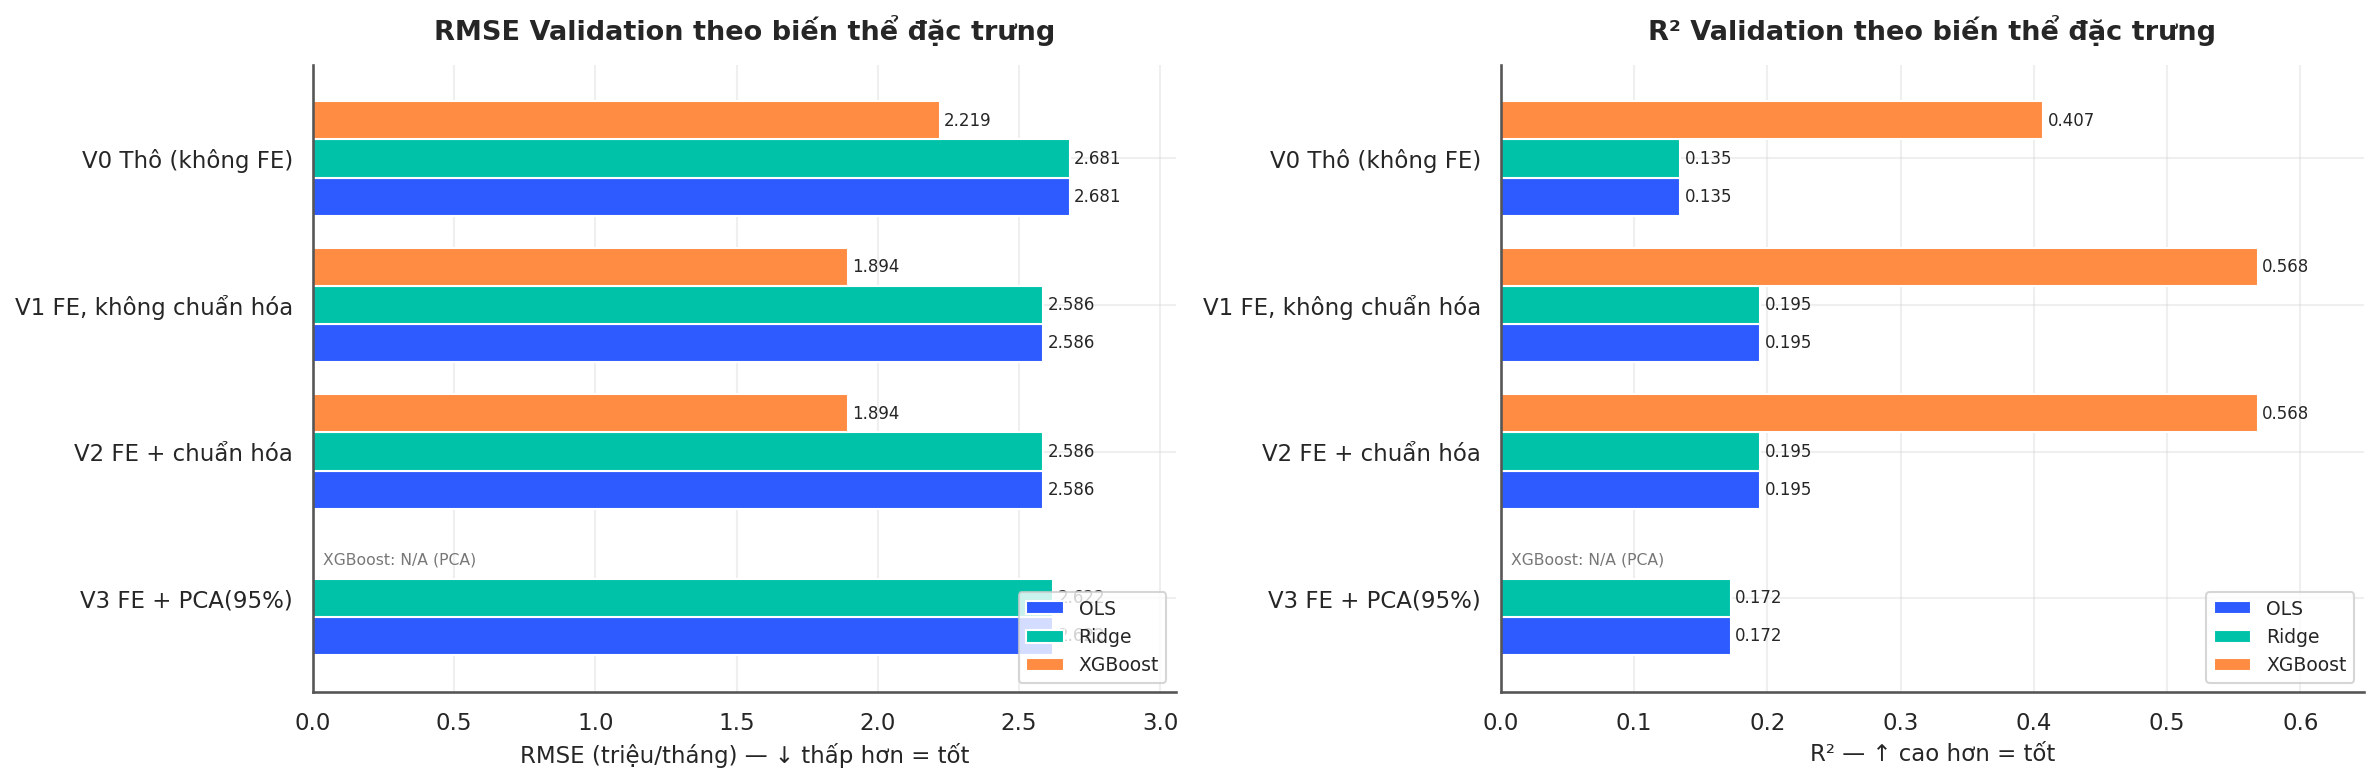
\includegraphics[width=0.90\textwidth]{abl_04_fe_pca}
  \caption{Thực nghiệm A — RMSE và R\textsuperscript{2} theo 4 biến thể đặc trưng}
  \label{fig:abl_fe}
\end{figure}

\textbf{Kết luận và quyết định:}
{\sloppy
\begin{itemize}[leftmargin=*, itemsep=2pt]
  \item \textbf{Dùng FE (V2):} tách \texttt{city}\slash\texttt{district} từ \texttt{full\_address}
        giảm RMSE \textbf{3.5\% (tuyến tính) đến 14.6\% (XGBoost)} — nguồn cải thiện là
        \textit{mở khóa tín hiệu khu vực} ẩn trong chuỗi địa chỉ (đúng trọng tâm đề tài
        ``theo khu vực'').
  \item \textbf{Không dùng PCA:} $\approx$80 chiều sau One-Hot chưa đủ cao để PCA phát huy;
        nén về $\approx$95\% phương sai loại bỏ mất tín hiệu quận/huyện quan trọng → RMSE tuyến tính
        tệ hơn. Ngoài ra PCA \textbf{phá vỡ cấu trúc đặc trưng riêng lẻ} (gộp tiện ích/khu vực vào
        các thành phần chính) nên không phù hợp với mô hình cây triển khai (cột XGBoost N/A).
  \item \textbf{Giữ chuẩn hóa:} không đổi kết quả với OLS/XGBoost
        (bất biến co giãn tuyến tính), nhưng cần thiết cho Ridge/LASSO và PCA.
\end{itemize}
}

\fbox{\textbf{Quyết định A:} Pipeline dứt khoát dùng \textbf{FE + chuẩn hóa Z-score (V2)}.}

% ─────────────────────────────────────────────────────────────────
\subsection[Thực nghiệm B — Biến mục tiêu: price gốc vs. log1p(price)]{Thực nghiệm B — Biến mục tiêu: \texttt{price} gốc vs.\ $\log(1+\text{price})$}
\label{subsec:abl_log}

\textbf{Câu hỏi:} Log-transform biến mục tiêu có thực sự tăng hiệu năng, hay làm mô hình
``underweight'' phân khúc giá cao?
(Giá cao đều có nguyên nhân thực: vị trí trung tâm, đầy đủ tiện ích.)

\textbf{Thiết kế:} ngoài MAE/RMSE/R\textsuperscript{2} toàn cục, đo riêng
\textbf{bias phân khúc giá cao} ($\geq$10 triệu/tháng, 8.3\% Validation):
$\text{bias} = \overline{\hat{y} - y}$; âm nhiều = dự đoán hụt hệ thống.

\begin{table}[H]
  \centering
  \caption{Đối sánh mục tiêu — \texttt{price} gốc vs.\ $\log1p(\text{price})$}
  \label{tab:abl_log}
  \small
  \begin{tabular}{@{}l l r r r r@{}}
    \toprule
    \textbf{Mô hình} & \textbf{Mục tiêu} &
    \textbf{MAE} & \textbf{RMSE} & \textbf{R\textsuperscript{2}} &
    \textbf{Bias giá cao ($\geq$10tr)} \\
    \midrule
    OLS & \textbf{price gốc}  & 1.963 & \textbf{2.586} & \textbf{0.195} & $-5.61$ triệu \\
    OLS & log1p(price) & \textbf{1.882} & 2.636 & 0.164 & $-6.31$ triệu \\
    \addlinespace
    XGBoost & \textbf{price gốc}  & 1.256 & \textbf{1.894} & \textbf{0.568} & $-2.79$ triệu \\
    XGBoost & log1p(price) & \textbf{1.236} & 1.936 & 0.549 & $-3.33$ triệu \\
    \bottomrule
  \end{tabular}
\end{table}

\begin{figure}[H]
  \centering
  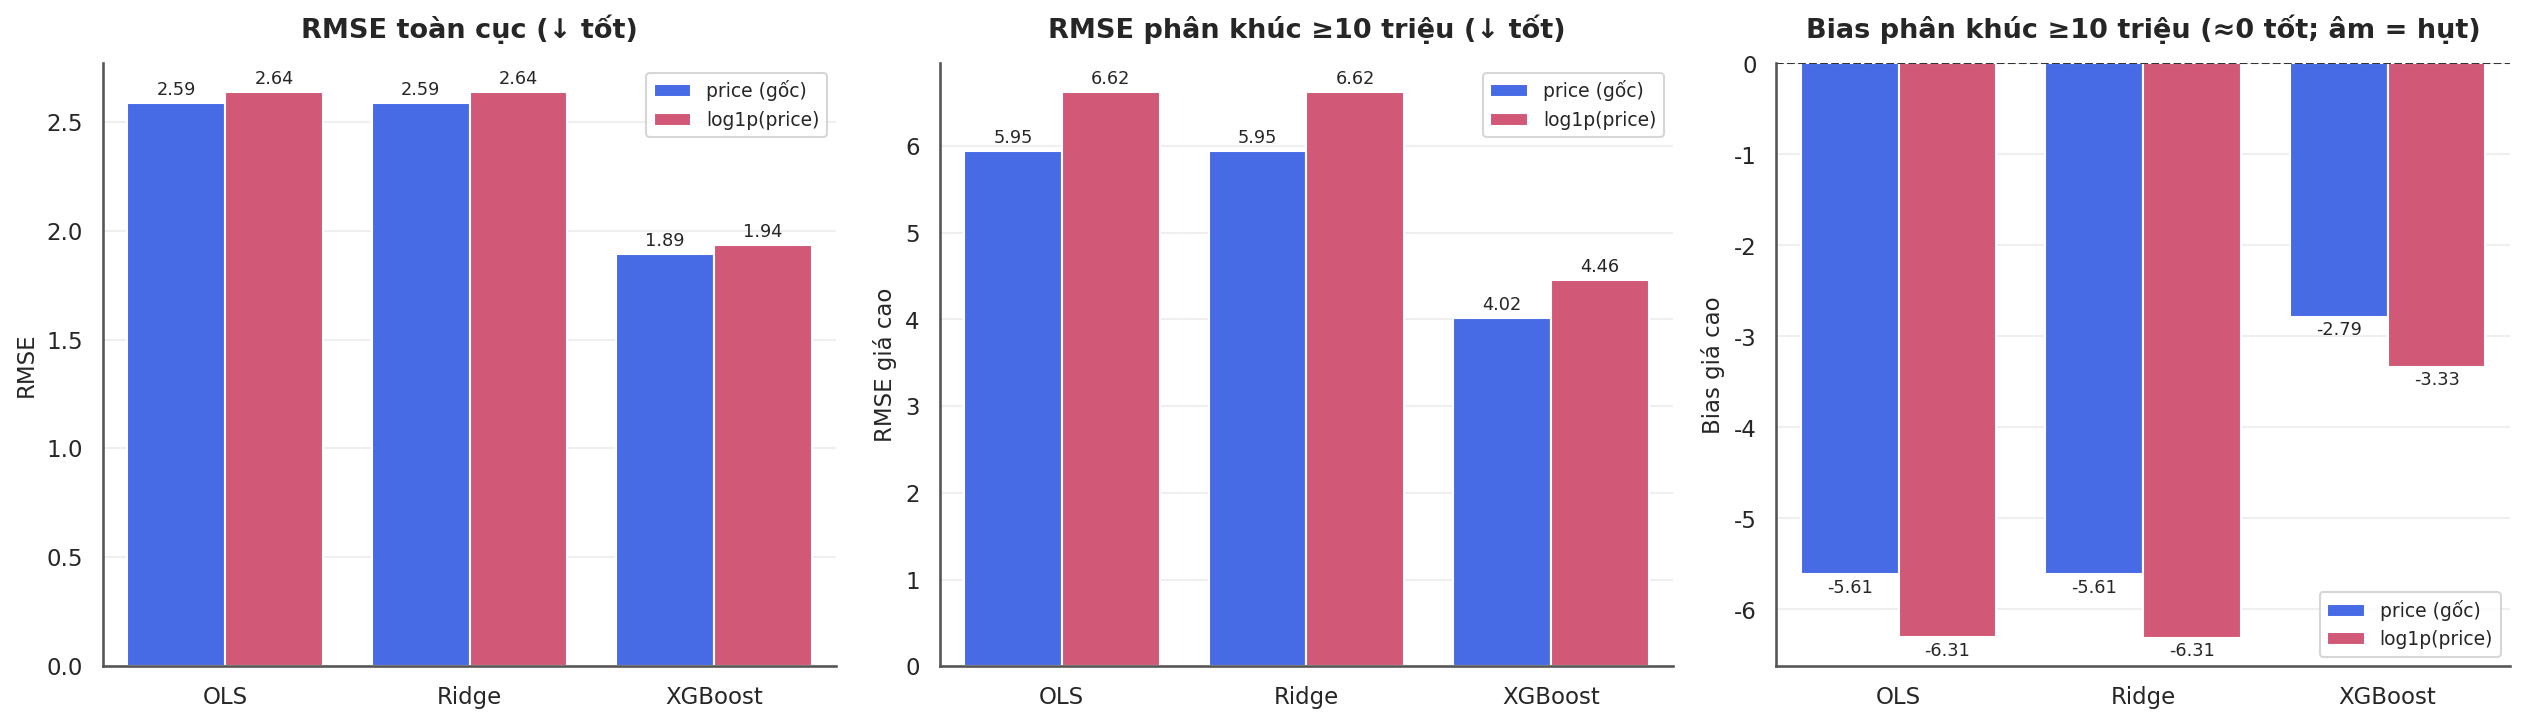
\includegraphics[width=0.90\textwidth]{abl_05_log_target}
  \caption{Thực nghiệm B — RMSE toàn cục (trái), RMSE phân khúc giá cao (giữa),
           Bias giá cao (phải)}
  \label{fig:abl_log}
\end{figure}

\textbf{Kết luận và quyết định:}
\begin{itemize}[leftmargin=*, itemsep=2pt]
  \item Log cải thiện MAE $\approx$1.6--4.1\%, nhưng \textbf{RMSE tăng 1.9--2.2\%} và R\textsuperscript{2}
        giảm — không cải thiện theo tiêu chí chọn mô hình chính (RMSE).
  \item \textbf{Bias phân khúc giá cao âm sâu hơn:}
        OLS $-5.61 \to -6.31$ triệu; XGBoost $-2.79 \to -3.33$ triệu.
        Đúng hiện tượng \textit{underweight}: log nén phân khúc giá cao, làm mô hình
        đánh giá thấp các căn hộ đắt dù chúng có nguyên nhân giá thực sự.
  \item Gợi ý log từ phân tích phân phối (EDA) \textbf{bị thực nghiệm bác bỏ}.
\end{itemize}

\fbox{\textbf{Quyết định B:} Cả 5 mô hình huấn luyện trực tiếp trên \textbf{\texttt{price} gốc}.}

% ─────────────────────────────────────────────────────────────────
\subsection{Thực nghiệm C — Tác động của ngoại lệ trong tập huấn luyện}
\label{subsec:abl_outlier}

\textbf{Câu hỏi:} Nếu giữ lại ngoại lệ (giá tới 10.000 triệu $\approx$ 10 tỷ/tháng,
diện tích tới 1.000 m\textsuperscript{2}), hiệu năng trên vùng giá mục tiêu thay đổi thế nào?

\textbf{Thiết kế:} hai mô hình XGBoost hoàn toàn giống nhau, chỉ khác tập Train
(có / không có 6.8\% ngoại lệ);
chấm trên cùng tập Validation vùng mục tiêu (\texttt{price}$\leq$17, \texttt{area}$\leq$180).

\begin{table}[H]
  \centering
  \caption{XGBoost — cùng Validation vùng mục tiêu, chỉ khác tập Train}
  \label{tab:abl_out}
  \begin{tabular}{@{}l c c@{}}
    \toprule
    \textbf{Tập Train} & \textbf{RMSE Validation} & \textbf{So với pipeline chính} \\
    \midrule
    Có ngoại lệ (6.8\% outlier) & 8.956 & $+376\%$ \\
    \textbf{Đã lọc ngoại lệ (pipeline chính)} & \textbf{1.882} & — \\
    \bottomrule
  \end{tabular}
\end{table}

\begin{figure}[H]
  \centering
  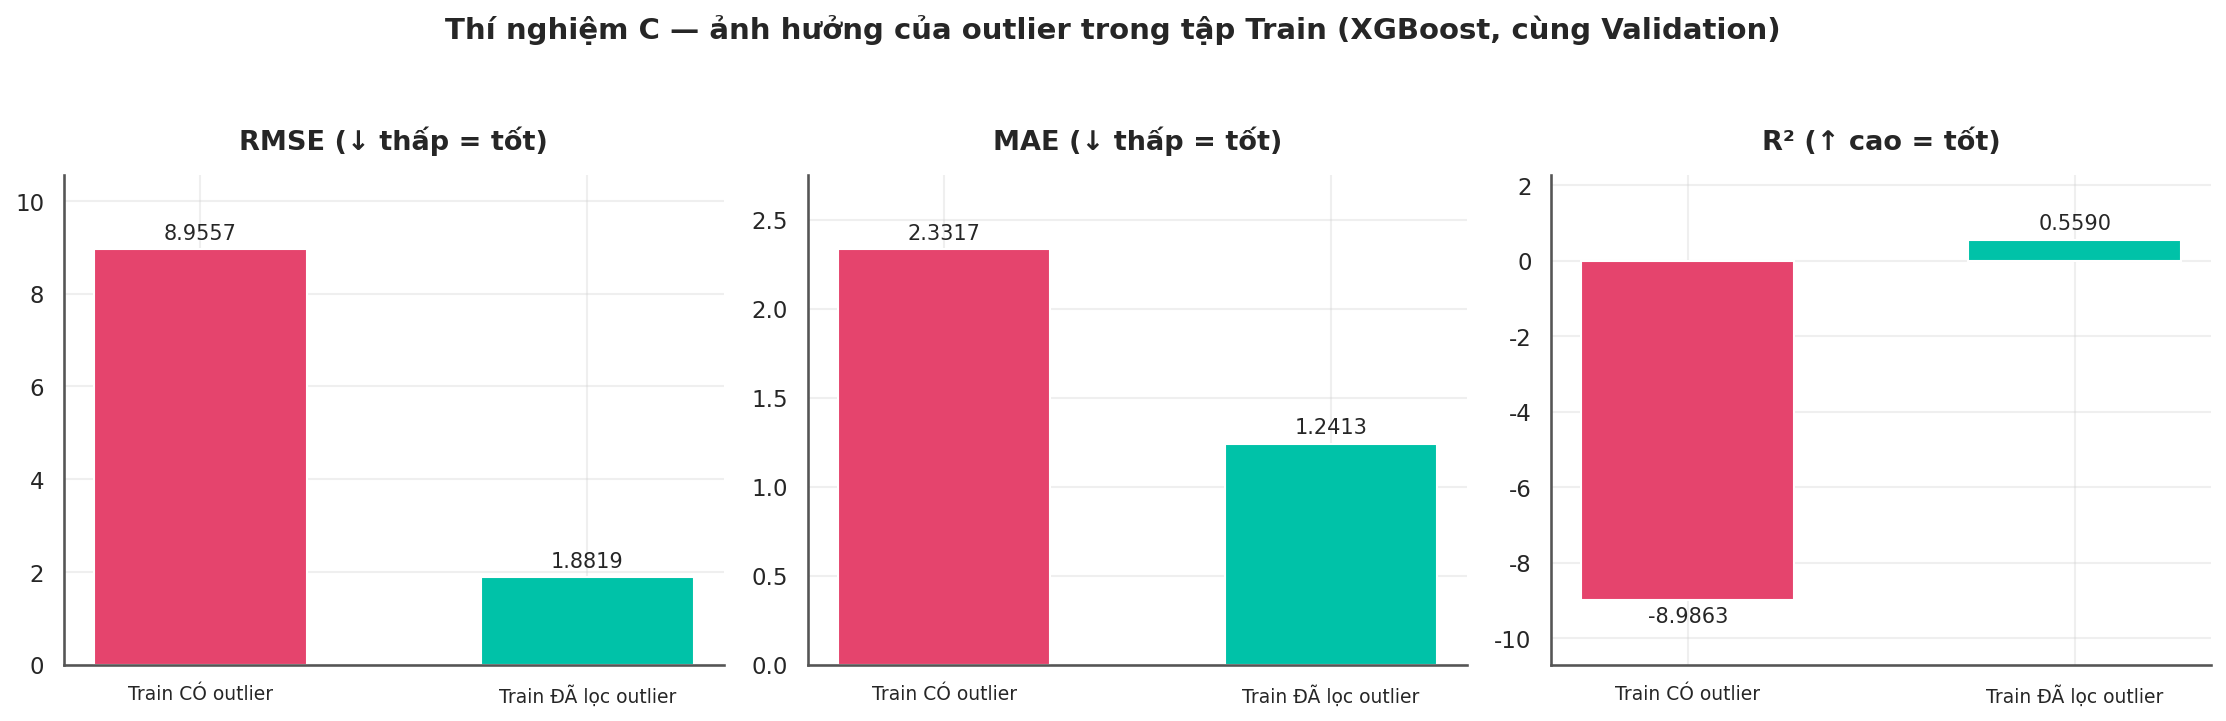
\includegraphics[width=0.90\textwidth]{abl_06_outliers}
  \caption{Thực nghiệm C — RMSE của XGBoost có / không outlier trong Train}
  \label{fig:abl_out}
\end{figure}

\textbf{Kết luận và quyết định:}
Giữ lại bản ghi giá hàng tỷ/tháng kéo lệch hàm mất mát bình phương —
mô hình phân bổ năng lực học cho vùng giá không bao giờ xuất hiện trong thực tế.
Lọc ngoại lệ giảm RMSE \textbf{79.0\%} trên vùng mục tiêu.

\fbox{\textbf{Quyết định C:} \textbf{Lọc outlier} (\texttt{price}$\leq$17, \texttt{area}$\leq$180) trước khi huấn luyện.}

% ─────────────────────────────────────────────────────────────────
\subsection{Tổng hợp quyết định pipeline}
\label{subsec:pipeline_summary}

Sau 3 thực nghiệm đối sánh, \textbf{pipeline dứt khoát} được xác định:

\begin{table}[H]
  \centering
  \caption{Tổng hợp 3 quyết định thiết kế pipeline — có kiểm chứng thực nghiệm}
  \label{tab:pipeline}
  \begin{tabularx}{\textwidth}{@{}l X l@{}}
    \toprule
    \textbf{Quyết định} & \textbf{Lý do (từ số liệu)} & \textbf{Thực nghiệm} \\
    \midrule
    FE: tách \texttt{city}/\texttt{district} & Giảm RMSE 3.5--14.6\%; PCA không giúp ích & A \\
    Mục tiêu: \texttt{price} gốc & Log tăng RMSE + underweight giá cao & B \\
    Lọc outlier: price$\leq$17, area$\leq$180 & Không lọc làm RMSE $\times$4.8 & C \\
    \bottomrule
  \end{tabularx}
\end{table}

\textbf{Kết quả ở Mục~\ref{subsec:main_results} dưới đây được tính trên pipeline sau
quyết định A--C} (so sánh họ mô hình và chọn mô hình triển khai).

% ─────────────────────────────────────────────────────────────────
\subsection{Kết quả chính: 10-fold CV và đánh giá Test}
\label{subsec:main_results}

5 mô hình được huấn luyện và đánh giá với \textbf{pipeline đã được xác nhận} ở Mục~\ref{subsec:pipeline_summary}:
dùng FE (city/district), mục tiêu \texttt{price} gốc, dữ liệu đã lọc ngoại lệ.

\begin{table}[H]
  \centering
  \caption{So sánh 5 mô hình — 10-fold CV (Train+Val) và đánh giá Test 1 lần duy nhất.
           $\star$ = mô hình triển khai.}
  \label{tab:model_compare}
  \begin{tabular}{@{}l r@{$\;\pm\;$}l r r r r@{}}
    \toprule
    \textbf{Mô hình} &
    \multicolumn{2}{c}{\textbf{CV RMSE}} &
    \textbf{CV R\textsuperscript{2}} &
    \textbf{Test MAE} & \textbf{Test RMSE} & \textbf{Test R\textsuperscript{2}} \\
    \midrule
    OLS           & 2.582 & 0.018 & 0.193 & 1.958 & 2.586 & 0.190 \\
    Ridge         & 2.582 & 0.018 & 0.193 & 1.958 & 2.586 & 0.190 \\
    LASSO         & 2.587 & 0.019 & 0.190 & 1.961 & 2.589 & 0.188 \\
    Random Forest & 2.112 & 0.029 & 0.460 & 1.380 & 2.114 & 0.459 \\
    \midrule
    \textbf{XGBoost} $\star$
      & \textbf{1.881} & 0.007 & \textbf{0.572} & \textbf{1.256} & \textbf{1.895} & \textbf{0.565} \\
    \bottomrule
  \end{tabular}
\end{table}

\begin{figure}[H]
  \centering
  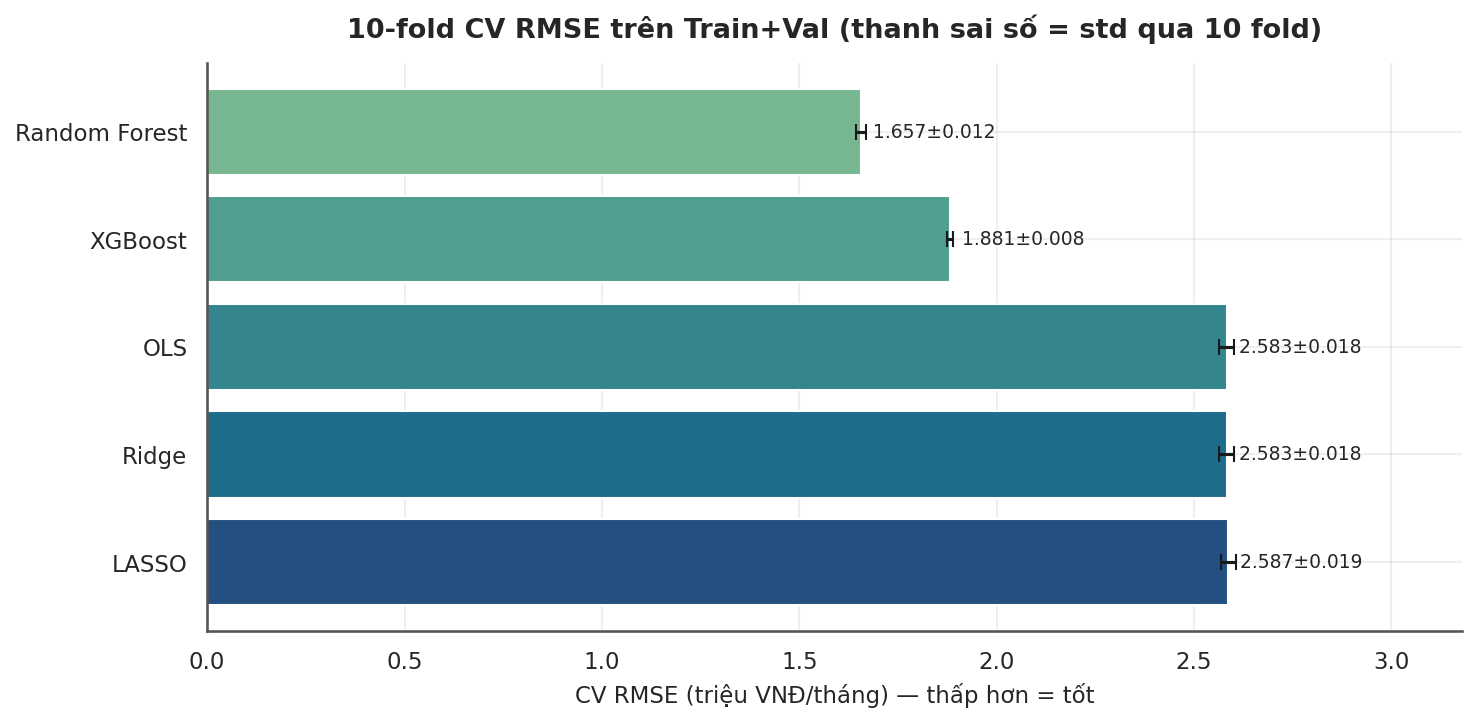
\includegraphics[width=0.86\textwidth]{eval_01_cv_rmse_comparison}
  \caption{CV RMSE của 5 mô hình (mean $\pm$ std, 10 fold)}
  \label{fig:cv_compare}
\end{figure}

\begin{figure}[H]
  \centering
  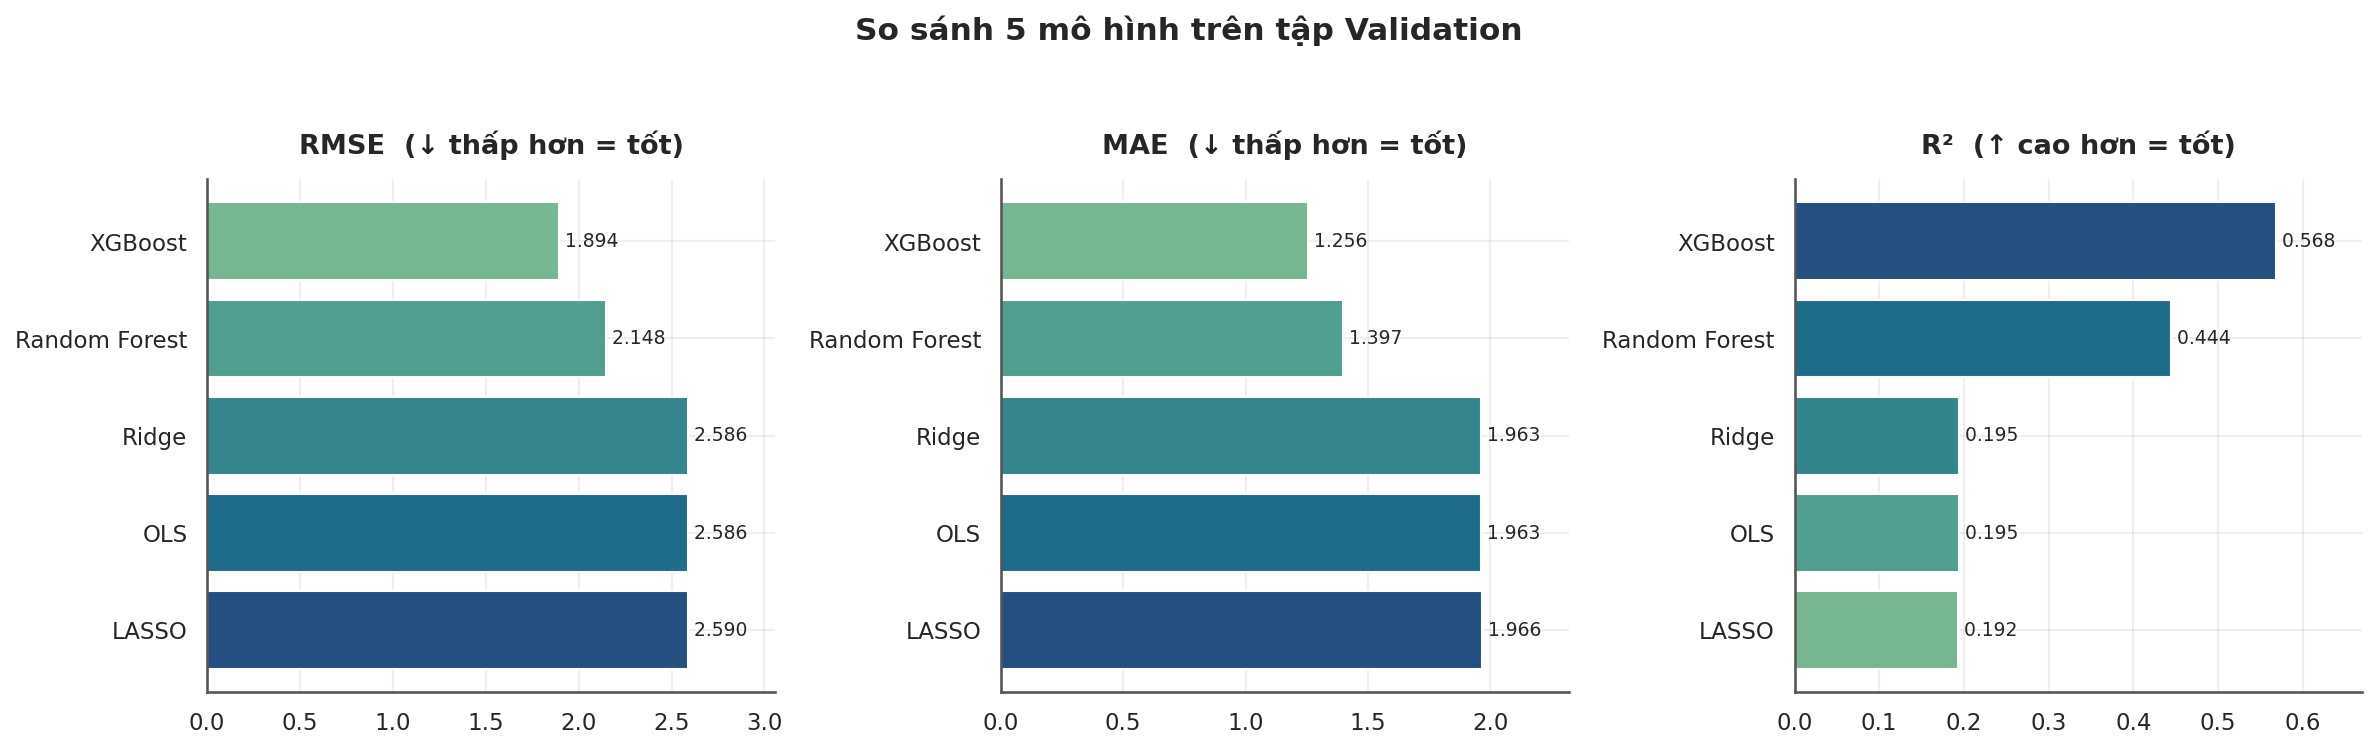
\includegraphics[width=0.86\textwidth]{model_01_model_comparison_val}
  \caption{So sánh RMSE, MAE và R\textsuperscript{2} của 5 mô hình trên tập Validation}
  \label{fig:val_compare}
\end{figure}

\textbf{Phân tích kết quả:}
\begin{itemize}[leftmargin=*, itemsep=3pt]
  \item Mô hình cây \textbf{vượt trội rõ rệt} so với tuyến tính
        (Test R\textsuperscript{2}: $\approx$0.46--0.57 vs.\ $\approx$0.19),
        xác nhận quan hệ phi tuyến và tương tác khu vực $\times$ diện tích
        được gợi ý từ PCA ở Mục~\ref{subsec:clustering}.
  \item CV RMSE $\approx$ Test RMSE, std nhỏ $\Rightarrow$ mô hình \textbf{không overfit},
        khái quát hóa tốt.
  \item \textbf{So sánh công bằng — cả Random Forest lẫn XGBoost đều áp ràng buộc đơn điệu}
        (tick tiện ích không làm giảm giá dự báo; xem Mục~\ref{sec:method}). Dưới cùng ràng buộc,
        \textbf{XGBoost chính xác hơn hẳn Random Forest} (Test R\textsuperscript{2} $0.565$ vs.\
        $0.459$; RMSE $1.895$ vs.\ $2.114$): boosting cộng dồn ``trải'' ràng buộc qua nhiều cây nên
        mất ít độ khớp, còn Random Forest (bagging) ép ràng buộc cứng trên từng cây độc lập rồi mới
        trung bình nên suy giảm mạnh hơn nhiều.
  \item \textbf{Mô hình triển khai là XGBoost} — nay là lựa chọn tốt nhất trên \textbf{cả hai}
        phương diện:
        \begin{enumerate}[leftmargin=1.2em, itemsep=1pt, topsep=2pt]
          \item \textbf{Chính xác nhất} trong nhóm mô hình có ràng buộc (Test R\textsuperscript{2}
                = 0.565, RMSE = 1.895).
          \item \textbf{Gọn nhẹ và triển khai nhanh:} XGBoost $\approx$0.86 MB so với Random Forest
                $\approx$56 MB ($n=500$ cây) — nằm gọn trong giới hạn GitHub ($<$100 MB), nạp/dự báo
                nhanh trong app Streamlit, lại có \textbf{early stopping} (regularization L1/L2 + tự
                dừng số cây).
        \end{enumerate}
        Khác với cách hiểu ``đánh đổi độ chính xác lấy triển khai'', ở đây \textbf{không có đánh
        đổi}: khi so công bằng, XGBoost vừa chính xác nhất vừa dễ triển khai nhất.
\end{itemize}

% ─────────────────────────────────────────────────────────────────
\subsection{Biểu đồ chẩn đoán mô hình triển khai (XGBoost)}
\label{subsec:diagnostics}

\begin{figure}[H]
  \centering
  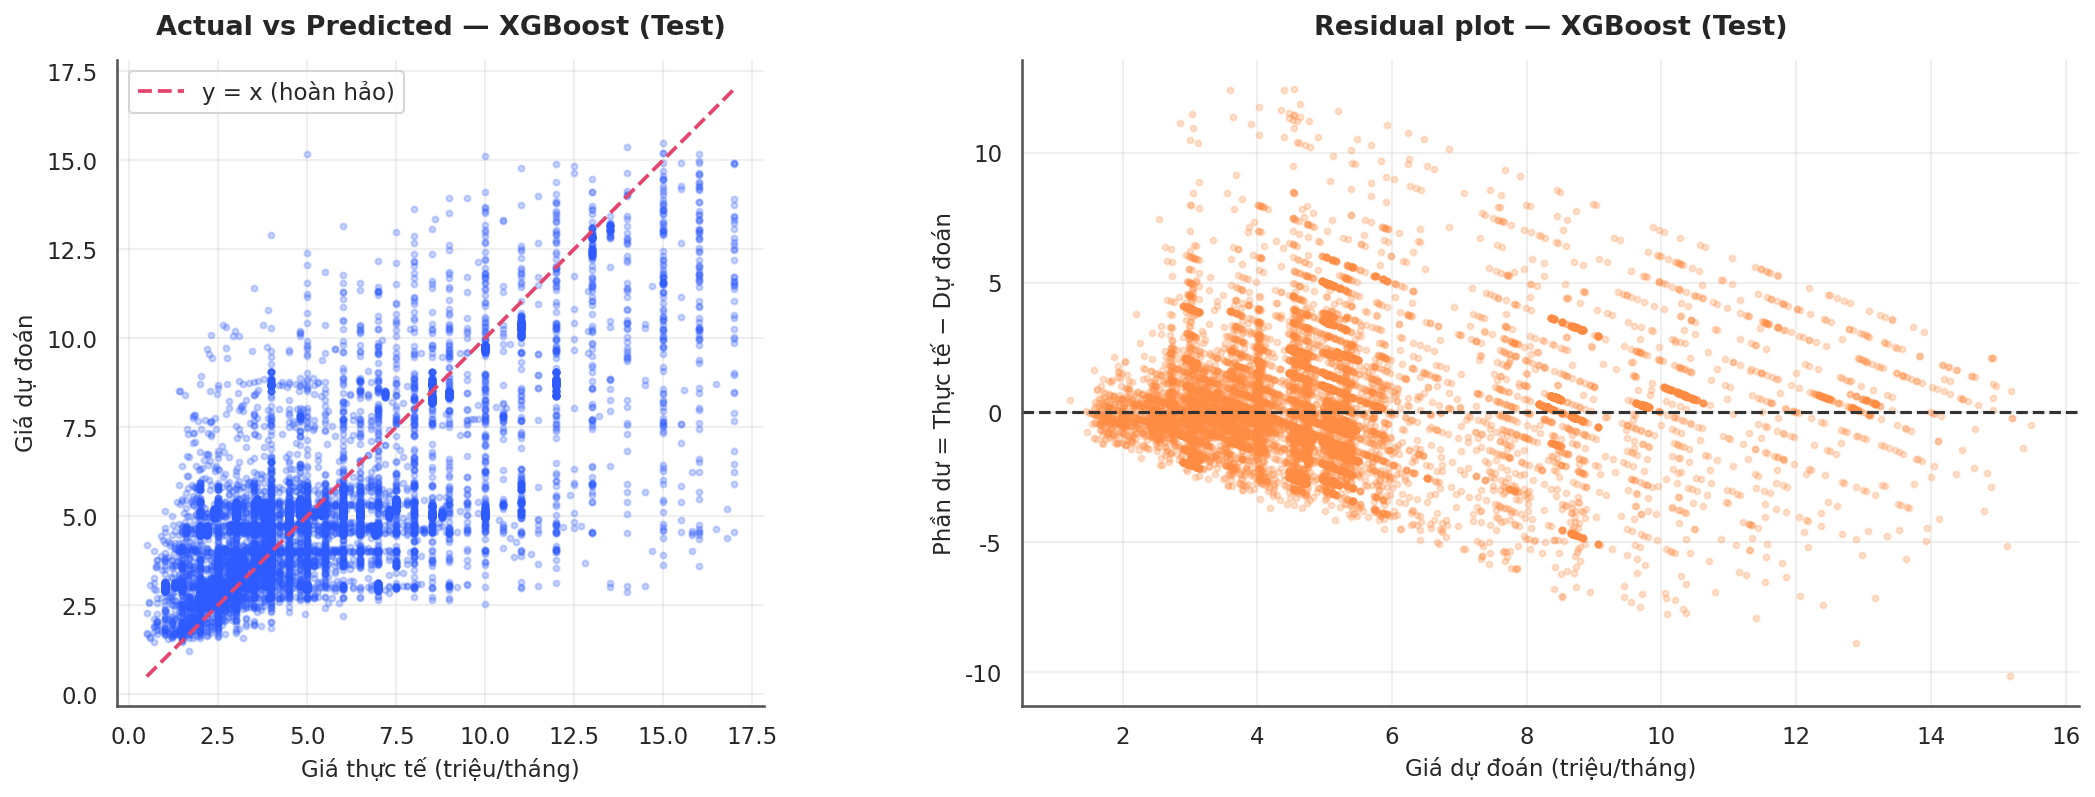
\includegraphics[width=0.86\textwidth]{eval_02_test_actual_vs_pred}
  \caption{Test — Actual vs Predicted (trái) và Residual vs Predicted (phải)}
  \label{fig:test_pred}
\end{figure}

\noindent \textbf{Nhận xét.} Điểm bám sát đường $y=x$, phần dư phân tán quanh 0
(mean $\approx$0) ở vùng giá phổ biến; riêng phân khúc giá cao mô hình có xu hướng
\textit{dự báo hụt} nhẹ (xem learning curve — bias).

\begin{figure}[H]
  \centering
  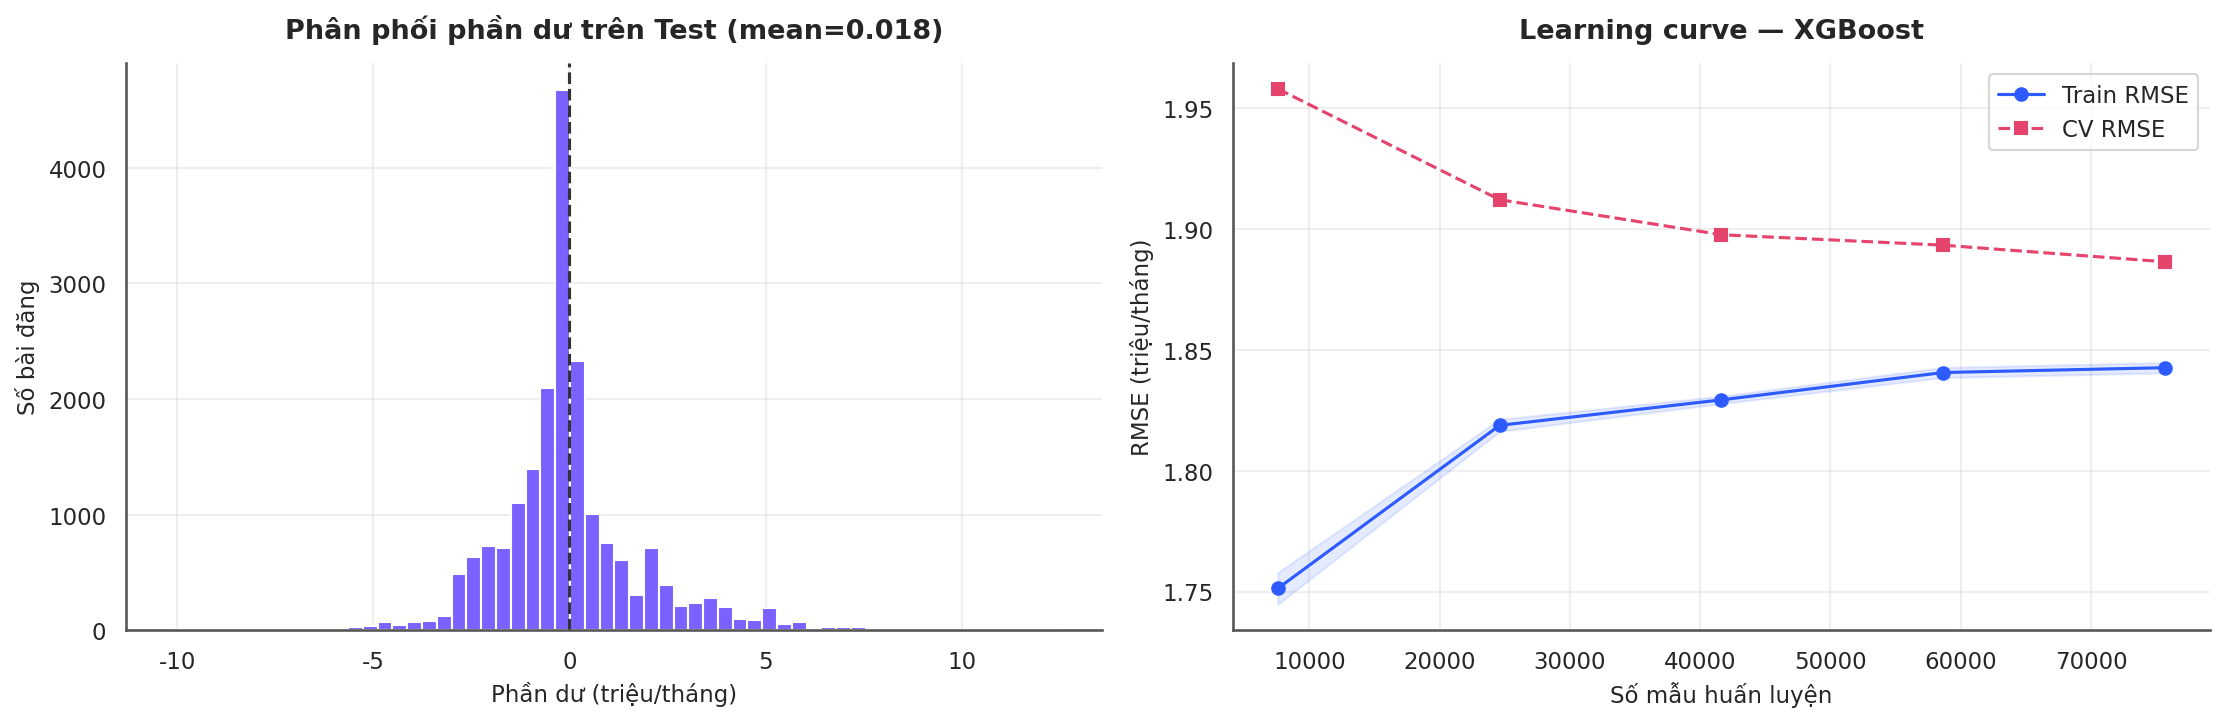
\includegraphics[width=0.86\textwidth]{eval_03_residual_learning_curve}
  \caption{Phân phối phần dư (trái) và Learning curve (phải)}
  \label{fig:lc}
\end{figure}

\noindent \textbf{Nhận xét.} Train RMSE và CV RMSE hội tụ khi tăng dữ liệu
$\Rightarrow$ không overfit nặng; khoảng cách còn lại là \textit{bias} — cần bổ sung
đặc trưng mới (GPS, NLP mô tả).

\begin{figure}[H]
  \centering
  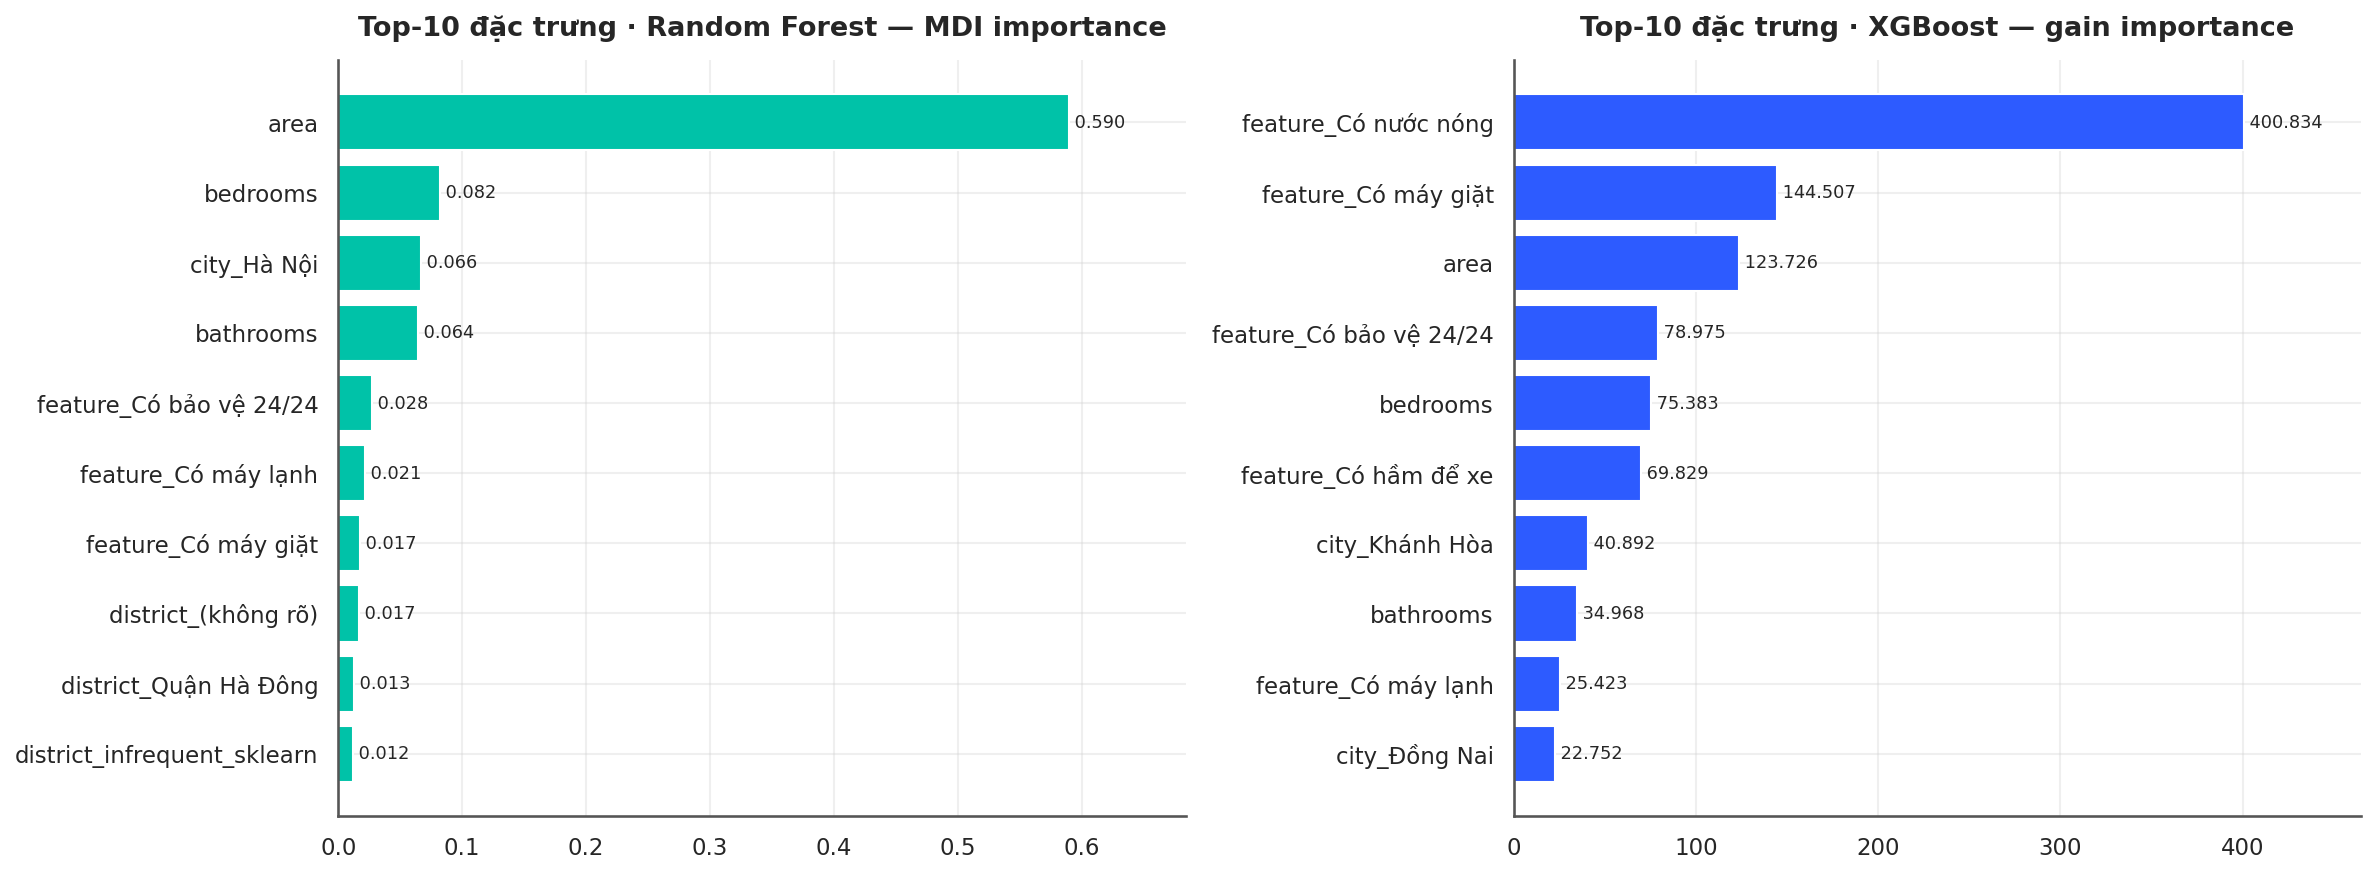
\includegraphics[width=0.84\textwidth]{model_02_feature_importance}
  \caption{Feature Importance — RF (MDI, trái) và XGBoost (total gain, phải)}
  \label{fig:importance}
\end{figure}

\noindent \textbf{Nhận xét.} Sau khi loại \texttt{source}, cả hai mô hình đều cho thấy
\texttt{area} là đặc trưng quan trọng nhất và vượt trội rõ rệt. Với Random Forest,
\texttt{area} đứng đầu với MDI $0.468$, tiếp theo là các tiện ích như
\texttt{feature\_Có hầm để xe}, \texttt{feature\_Có nước nóng} và số phòng ngủ
(\texttt{bedrooms}). Với XGBoost, theo thước đo \textit{total gain} chuẩn hóa,
\texttt{area} cũng dẫn đầu với giá trị $0.532$, sau đó là \texttt{bedrooms},
\texttt{feature\_Có nước nóng} và \texttt{bathrooms}. Nhìn chung, dù thứ tự các đặc trưng có khác nhau giữa hai mô hình, cả hai đều xác nhận diện tích, số phòng và nhóm tiện ích là các yếu tố chính ảnh hưởng đến giá thuê. Điều này phù hợp với kỳ vọng thực tế và cho thấy các đặc trưng được tạo thêm trong bước FE có đóng góp đáng kể cho mô hình.